\documentclass[UTF8,a4paper,10pt,nocolorlinks]{ctexart}
\usepackage[left=2.50cm, right=2.50cm, top=2.50cm, bottom=2.50cm]{geometry} %页边距
\CTEXsetup[format={\Large\bfseries}]{section} %设置章标题居左   
\usepackage{ctex}
\CTEXoptions[today=old]
\usepackage{cite}
% 代码块儿
\usepackage{textcomp} % 必须加上,否则报错
\usepackage{listings}
\usepackage{xcolor}
% \usepackage{fontspec}
% \setmonofont{Consolas}
\usepackage{varioref}       % ref 跨页调用
\usepackage{ctex}
\usepackage{multicol}
\usepackage{amssymb}        % 等于号 上面 加一个三角形
\usepackage{setspace}
\usepackage{tikz} % package used for the tikz
\usepackage{mdframed}
\usepackage{titletoc}
\usepackage{etoolbox}

\usepackage{helvet}
\usepackage{caption}
\usepackage{multicol} %用于实现在同一页中实现不同的分栏
\usepackage{changepage}
\usepackage{graphics}
\usepackage{amsmath, amsfonts, amssymb} % math equations, symbols
\usepackage[english]{babel}
\usepackage{color}      % color content
\usepackage{graphicx}   % import figures
\usepackage{url}        % hyperlinks
\usepackage{bm}         % bold type for equations
\usepackage{multirow}
\usepackage{booktabs}
\usepackage{epstopdf}
\usepackage{epsfig}
\usepackage{algorithm}
\usepackage{algorithmic}

\usepackage[pagestyles]{titlesec}
% \renewcommand{\algorithmicrequire}{ \textbf{Input:}}     % use Input in the format of Algorithm  
% \renewcommand{\algorithmicinput}{ \textbf{Input:}}     % use Input in the format of Algorithm  
\renewcommand{\algorithmicensure}{ \textbf{Input:}} % use Initialize in the format of Algorithm  
% \renewcommand{\algorithmicreturn}{ \textbf{Output:}}     % use Output in the format of Algorithm  
\renewcommand{\figurename}{图}
% 引用参考文献标号显示在右上角
\newcommand{\upcite}[1]{\textsuperscript{\textsuperscript{\cite{#1}}}}

\newpagestyle{teststyle}{
  \sethead{学号: 2019520941}{\sectiontitle}{第\thepage页}
  \renewcommand{\makeheadrule}{
    \makebox[0pt][l]{\rule[-.3\baselineskip]{\linewidth}{.5pt}}
    \rule[-.4\baselineskip]{\linewidth}{.5pt}
  }
}
\usepackage{color}
\usepackage{subfigure}
\usepackage{changepage}
\usepackage{fancyhdr} %设置页眉、页脚
\pagestyle{fancy}  %%%单线页眉
\fancyhead{}
\fancyhead[LO]{A*算法和模拟退火算法无人机领域的应用}
\fancyhead[RO]{冯学伟}
% \fancyfoot[RO]{\thepage}
\fancypagestyle{plain}{%
  \pagestyle{fancy}
}
\usepackage{shorttoc}
\usepackage{xcolor}
\usepackage{mdframed}
\usepackage{titletoc}
% \renewcommand{\today}{\CJKnumber\year 年 \CJKnumber\month 月 \CJKnumber\day 日}

\DeclareRobustCommand{\chuhao}{\fontsize{42pt}{\baselineskip}\selectfont}  % 初号
\DeclareRobustCommand{\xiaochu}{\fontsize{36pt}{\baselineskip}\selectfont} % 小初
\DeclareRobustCommand{\yihao}{\fontsize{26pt}{\baselineskip}\selectfont}   % 一号
\DeclareRobustCommand{\xiaoyi}{\fontsize{24pt}{\baselineskip}\selectfont}  % 小一
\DeclareRobustCommand{\erhao}{\fontsize{22pt}{\baselineskip}\selectfont}   % 二号
\DeclareRobustCommand{\xiaoer}{\fontsize{18pt}{\baselineskip}\selectfont}  % 小二
\DeclareRobustCommand{\sanhao}{\fontsize{16pt}{\baselineskip}\selectfont}  % 三号 
\DeclareRobustCommand{\xiaosan}{\fontsize{15pt}{\baselineskip}\selectfont} % 小三
\DeclareRobustCommand{\sihao}{\fontsize{14pt}{\baselineskip}\selectfont}   % 四号
\DeclareRobustCommand{\xiaosi}{\fontsize{12pt}{\baselineskip}\selectfont}  % 小四
\DeclareRobustCommand{\wuhao}{\fontsize{10.5pt}{\baselineskip}\selectfont} % 五号
\DeclareRobustCommand{\xiaowu}{\fontsize{9pt}{\baselineskip}\selectfont}   % 小五
\DeclareRobustCommand{\liuhao}{\fontsize{7.5pt}{\baselineskip}\selectfont} % 六号
\DeclareRobustCommand{\xiaoliu}{\fontsize{6.5pt}{\baselineskip}\selectfont}% 小六
\DeclareRobustCommand{\qihao}{\fontsize{5.5pt}{\baselineskip}\selectfont}  % 七号

\lstset{numbers=left,numberstyle=\tiny,
breaklines=true,  %代码过长则换行
keywordstyle=\color{blue!70},commentstyle=\color{red!50!green!50!blue!50},frame=shadowbox, rulesepcolor=\color{gray!20!green!20!blue!20},escapeinside=``,xleftmargin=2em,xrightmargin=2em, aboveskip=1em}

\providecommand{\keywords}[1]{\textbf{\textit{keywords---}} #1}

 
\usepackage{hyperref} %bookmarks
% \usepackage[colorlinks,linkcolor=red,anchorcolor=blue,citecolor=green,CJKbookmarks=True]{hyperref}
\hypersetup{colorlinks, bookmarks, unicode} % unicode
 
\captionsetup[figure]{labelfont={bf},labelformat={default},labelsep=period,name={图}}
\newenvironment{figurehere}
{\def\@captype{figure}}
{}
 
% \title{\textbf{A*算法和模拟退火算法无人机领域的应用}}
% \author{ 冯学伟 \thanks{学号:2019520941}}
% \date{\today}

%标题、作者及日期
% \huge{\textbf{无人机导航控制}}\\[3mm]
% \Large{\textbf{The Navigational Control In The Field Of Unmanned Air Vehicle}}\\[1mm]
\title{
    \huge{\textbf{无人机导航控制}}\\
    \Large{\textbf{The Navigational Control In The Field Of Unmanned Air Vehicle}}
}

\author{冯学伟}
\date{\today}

\begin{document}
    % \maketitle
    %%%%%%%%%%%%%%%%%%%%%%%%%% 封面 <<<<<<<< %%%%%%%%%%%%%%%%%%%%%%%%%%
    \begin{figure}[t]
		\parbox[b]{2cm}{
			\includegraphics[width=\textwidth]{TYUT.jpg}
			}
	\end{figure}

	\begin{center}
		\quad \\
		\quad \\
		\heiti \fontsize{45}{17} 课\quad 程\quad 论\quad 文
		\vskip 3.5cm	
        \begin{center} % Application in the field of drones
            \huge{\textbf{无人机导航控制}}\\[3mm]
            \Large{\textbf{The Navigational Control In the Field Of Unmanned Air Vehicle}}\\[1mm]
        \end{center}
	\end{center}
    \vskip 3.5cm
    
    \begin{quotation}
        \begin{center}
            \begin{flushleft}
            \songti \fontsize{15}{15}
            \doublespacing
            \par\setlength\parindent{12em}
            \quad 
            \sanhao 
            \centering
            \begin{tabular}{cc}
                学\hspace{1.2cm}  院:&\underline{\qquad\  软件学院 \ \qquad}\\
                专\hspace{1.2cm}  业:&\underline{\qquad\  软件工程 \ \qquad}\\
                学生姓名:&\underline{\qquad\quad 冯学伟 \quad\qquad}\\
                学\hspace{1cm} 号:&\underline{\quad\quad 2019520941 \quad\quad}\\
                指导教师:&\underline{\qquad\quad 谢红薇  \quad\qquad}\\
                时\hspace{1cm} 间:&\underline{\quad2020年5月19日\qquad}\\
            \end{tabular}
            \vskip 2cm
            \centering
            \end{flushleft}
        \end{center}
	\end{quotation}
    \thispagestyle{empty} % 设置当前页 页版式
    \clearpage
    %%%%%%%%%%%%%%%%%%%%%%%%%% <<<<<<<< 封面 %%%%%%%%%%%%%%%%%%%%%%%%%%


    %%%%%%%%%%%%%%%%%%%%%%%%%%%%%%%%%%%%%%%%%%%%%%%%%%%%%%%%% 目录 %%%%
    \renewcommand{\contentsname}{目录}  % 将Contents改为目录
    \tableofcontents
    \thispagestyle{empty} % 设置当前页 页版式
    \clearpage % 分页/
    %%%%%%%%%%%%%%%%%%%%%%%%%%%%%%%%%%%%%%%%%%%%%%%%%%%%%%%%% 目录 %%%%


    %  \thispagestyle{empty}       %本页不显示页码
     
    \renewcommand{\abstractname}{摘要}  % 将Abstract改为摘要
    \begin{center}
        \large{\textbf{摘要}}
    \end{center}
    \begin{adjustwidth}{0cm}{0cm}
        \hspace{2em} 无人飞行器(UnmannedAirVehicle.UAV)具有广阔的应用前景,是近年来高技术研究的热点目标之一。随着计算机技术,通信技术,传感器技术,电池技术等的
        飞速发展,开展微型UAV研究并把它运用到军事或民用中已经成为可能。本论文以PX4控制逻辑为基础,进行了一定的改进,实现了更加平滑的转弯控制,使得
        无人机能以更地高效率执行航线。
        \begin{flushleft}
        \par\textbf{关键字: } 无人机; 航线规划; PX4; 转弯逻辑 %“\par在段首,表示另起一行,“\textbf{}”,花括号内的内容加粗显示
        \end{flushleft}
    \end{adjustwidth}
    \thispagestyle{empty} % 设置当前页 页版式
    \clearpage

    \begin{center}
        \large{\textbf{Abstract}}
    \end{center}
    % adjustwidth \usepackage{changepage}
    \begin{adjustwidth}{0cm}{0cm}
        \hspace{1em} Unmanned Air Vehicle (Unmanned Air Vehicle.UAV) has broad application prospects and is one of the focuses of long-range high-tech research. Through computer technology, communication technology, sensor technology, battery technology, etc.
        Based on the PX4 control logic, this paper has made certain improvements and achieved more elaborate turn control, which has achieved rapid development. It has become possible to carry out micro UAV research and apply it to military or civilian use.
        Drones can execute routes with higher efficiency.
        % \noindent 首行缩进
    \end{adjustwidth}
    \begin{keywords}
        % \noindent 可以取消段落首行缩进
        \noindent Unmanned Air Vehicle; Path Manager; PX4; the turning logic     
    \end{keywords}
    \thispagestyle{empty} % 设置当前页 页版式
    \clearpage % 分页


    \setcounter{page}{1}        %从下面开始编页,页脚格式为导言部分设置的格式
    %%%%%%%%%%%%%%%%%%%%%%%% 分栏 %%%%%%%%%%%%%%%%%%
    \pagestyle{teststyle}
    % \begin{multicols}{2}
    \section{无人机发展概述}
    无人飞行器(Unmanned Air Vehicle.UAV)具有广阔的应用前景,是近年来高技术研究的热点目标之一。
    随着社会的发展和经济的进步,无人机的发展逐步趋
于成熟。无人机的应用有不同的场景和方式,例如,应用于
军事勘探和追踪,农药的无人喷洒,民用影像航拍等。以
2017 年发生飓风的波多黎各为例,利用最合理的方法向
该地投放物资. 同时也伴随着计算机技术,通信技术,传感器技术,电池技术等的
    飞速发展,开展微型UAV研究并把它运用到军事或民用中已经成为可能。
    本论文以PX4控制逻辑为基础,进行了一定的改进,实现了更加平滑的转弯控制,使得
    无人机能以更地高效率执行航线。\par
    无人机系统通常较有人机复杂。系统的基本组成主要包括无人机、地面控制站、
发射回收装置及地面数据终端。控制站通常提供三个工作站:完成任务控制、无人
机控制及图像分析。地面数据终端完成与无人机的信息交流。另外,有些无人机系
统还增加了卫星作为其系统的组成部分,增加GPS以提高无人机定位的精度。无人
机研究的关键技术包括:飞行器系统技术一用于预测故障的综合性管理系统和满足
故障容错要求的制导、导航和控制系统;人工智能技术一用于解决无人机的自主程
度问题;通信技术一宽带、大数据量的数据链技术可以使无人机远距离快速传递信
息,实施超视距控制.

    \section{无人机体系框架}
    本文探讨的主要内容包括固定翼姿态控制,飞行向导及自主导航等功能,
以层次化的观点来看,PX4由两个层次组成:一是飞行控制栈(flight stack),即自驾仪的软件解决方案,二是中间件,一种可以支持任意类型自主机器人的通用机器人中间件。
如图\ref{px4}所示。整个系统是反应式的。
\begin{figure}[H]
    \centering
    \includegraphics[width=0.6\textwidth]{picture/PX4_Architecture_1.png}
    \caption{px4体系框架}
    \label{px4}
\end{figure}
箭头显示了模块之间最重要的连接的信息流。 实际上,连接比所示的多得多,并且大多数模块都可以访问一些特定的数据(例如,用于参数)。
模块通过使用名为uORB的发布-订阅消息总线相互通信,
使用“发布-订阅”方案意味着:系统是被动的,它是异步的,在有新数据可用时将立即更新
所有操作和通讯都完全并行化, 系统组件可以以线程安全的方式从任何地方使用数据.
其中,uORB(Micro Object Request Broker,微对象请求代理器)是PX4/Pixhawk系统中非常重要且关键的一个模块,它肩负了整个系统的数据传输任务,所有的传感器数据、GPS、PPM信号等都要从芯片获取后通过uORB进行传输到各个模块进行计算处理。实际上uORB是一套跨「进程」 的IPC通讯模块。在Pixhawk中,所有的功能被独立以进程模块为单位进行实现并工作。而进程间的数据交互就由为重要,必须要能够符合实时、有序的特点。

% \begin{figurehere}
%     \includegraphics[width=0.5\textwidth]{picture/PX4_Architecture_1.png}
%     \caption{PX4}
%     \label{px4}
% \end{figurehere}
    \subsection{飞行控制栈}    
    飞行堆栈是用于自主无人机的制导,导航和控制算法的集合。 
    它包括用于固定翼,多旋翼和VTOL机身的控制器,以及用于姿态和位置的估计器。
图\ref{fight}显示了飞行堆栈的构建块的概述。它包含从传感器、RC输入和自动飞行控制(导航器)到电动机或伺服控制(执行器)的完整管道。
\begin{figure}[H]
    \centering
    \includegraphics[width=0.6\textwidth]{picture/fight_stack.png}
    \caption{fight stack}
    \label{fight}
\end{figure}
其中,estimator、controller 和 mixer 担当主要角色。
estimator 获取一个或多个传感器输入,对其进行组合,然后计算vehicle状态(例如,来自IMU传感器数据的姿态);
controller 是将设定值和测量或估计状态(过程变量)作为输入的组件,其目标是调整过程变量的值,使其与设定值匹配,输出是最终达到该设定点的校正。例如,位置控制器将位置设定值作为输入,过程变量是当前估计的位置,输出是将vehicle移向所需位置的姿态和推力设定点;
mixer 接受力指令(例如向右转)并将其转换为单独的电机指令,同时确保不超出某些限制,这种转换是特定于vehicle类型的,并且取决于各种因素,例如相对于重心的电动机布置或vehicle的旋转惯性。
本文主要对 controller 内部的算法进行了一定的改进。
    \section{控制器}
    控制器主要包括:导航控制器(navigator)、制导控制器(position controller)和姿态控制器(attitude controller)三层结构;同时,上层的输出也是下层的输入,之间紧密衔接,没有主次之分。
        \subsection{导航控制}
        导航就字面上说,就是引导航行的意思,而其确切的定义可表述为:导航是有目的地、安全有效地引导运动体(船只、潜艇、地面车辆以及飞机、宇宙飞船等)
        从一地到另一地的控制过程。
        所有导航系统的相关研究,都是为了解决三个基本的导航课题。这三个课题是:
        \begin{itemize}
            \item [(1)] 
                如何确定被导航对象的位置
            \item [(2)]
                如何确定被导航对象从一个位置到另一个位置前进的方向
            \item [(3)]
                如何确定距离(或者速度、时间)
        \end{itemize}
        \par对每个导航系统来说,就是利用导航手段不断确定被导航对象航行中的位置、方向、距离、时间和速度,这些通常称之为“导航参量”。
        在这些导航参量中,对慢速运动体来说或对于远距离航行来说,“位置”是关键。因为导航系统知道了“在哪儿”之后,就可以决定是继续保持当时的速度和航向,还
    是要作某种改变。因此,按传统的观点,导航系统从某种意义上说就是定位系统。
但是对于高速运动的导航对象来说,测量和判断之间的时间滞后,使得位置信息不
具有更多的意义。这种情况下,驾驶员最关心的导航参量就是“航向”和“距离”,以
决定“到终点或下一条航路点要经过的那条航线?还有多远”的问题:而如果交通密
度很高,还会产生这样的问题:“在这个时刻,我应该在哪里?我实际上在哪里?怎
样到达我应该到达的下一个位置上去?”因此,这时所需要的连续的、实时的驾驶信
息输出,以便通过制导计算机来实行自动操纵。
总之,由于导航的目的和对象的不同,要求解决的问题也会有所区别。但从根
本上说,导航就是为了提供航行中的位置、方向、距离和速度这些导航参量。因此,
导航的研究,就是要弄清楚这些导航参量的如何测量和如何运用;而导航的实践,
就是运用所得到的结果来保证运动体安全而有效地航行。
从所用技术来分,导航可分为惯性导航、雷达、卫星导航;导航台;从应用方式来分,可分为自丰导航和地面导航。上面的惯性导航和雷达为自主导航;导航台
为地面导航;而卫星导航是一种综合的导航手段。
\subsection{导航中的定位技术}
从上面可以知道,如何确定位置是导航需要解决的基本问题之一,而且传统的导航系统从某种意义上说就是一个定位系统,这说明了定位技术在导航过程中的重
要地位。
目前,对于地面移动目标的定位技术主要包括无线电定位技术、GPS导航定位技术、惯性导航定位技术。
\begin{itemize}
    \item [1)] 无线电定位技术 \par
        该种定位技术由超高频视距无线电系统构成的同步时序网络,采用跳频和时分
    多址技术,提供数百个地面和空中平台的实时位置轨迹。定位精度可达几十米内,
    缺点是建网成本太高,军事上应用居多.
    \item [2)] 惯性导航定位技术 \par
    惯性导航系统利用陀螺、加速度计等惯性元件,测量运动平台相对于惯性空间的线运动和角运动参数,在给定初始条件下,由计算机推算出平台的导航参数,以
    引导平台完成预定的航行或行驶任务。惯性导航的突出优点是,具有高度的自主性,不需要外界的帮助,就能独立完成导航任务。缺点是有自身无法避免的累积误差.
    \item [3)] 基于GPS系统的定位技术 \par
    该技术优点是定位精度高,定位半径可达十几米。目前没有一种传统的导航定位技术能够达到GPS这样的高精度、高速度、全天候和全球性的性能。
    其缺点是需要终端内置GPS接收机,定位精度受终端所在环境的影响较大,如用户在室内时,定位精度将降低,甚至无法完成定位。
\end{itemize}
\par 从以上介绍可知这些导航定位技术各有其优点和不足,无线电定位技术和GPS
导航定位技术可以获得高精度,但容易受到干扰;惯性导航定位装置是纯自主式的,但必须借助于里程计等定时进行校正,才能保证定位精度。
因此,目前地面平台往往采用两种或两种以上的导航装置组成综合导航定位系统。但是组合导航系统是以提高成本为代价的,目前国内,应用较多也比较实用的是结合GIS的地图匹配算法.
\par
导航需要解决的第二个问题是在当前位置已知的前提下,如何才能到达目的地,也即路径规划。在本文的研究中,主要是改进UAV执行直线和直线之间的切换逻辑,让其飞行出来的航线更加的平滑。
之外,也存在着直线和曲线之间的切换逻辑,不过由于时间原因,这一部分还没有进行改善,仍需不断研究探讨。
        \subsection{制导控制}
        制导是导引和控制飞行器按一定规律飞向目标或预定轨道的技术和方法。制导过程中,导引系统不断测定飞行器与目标或预定轨道的相对位置关系,发出制导信息传递给飞行器控制系统,以控制飞行。分有线制导、无线电制导、雷达制导、红外制导、激光制导、音响制导、地磁制导、惯性制导和天文制导等。
        如果说导航是给出航线,引导目标到达某点,那么制导就是导引并控制目标到达某点。区别就像别人问路,导航就是给他指路,制导就是给他带路
        导航的对象范围比较大,通常用他的狭义定义指的是载具设备,但是广义定义下也能对人;制导的对象则范围小,通常用的狭义定义专指武器(导弹,制导炸弹,鱼雷),广义下也加入了飞行器
        \subsection{姿态控制}
        姿态控制器使用级联回路方法工作, 如图\ref{atti}所示。外环计算姿态设定值和估计姿态之间的误差,该误差乘以增益(P控制器)可生成速率设定点。然后,内部循环计算速率误差,并使用PI(比例+积分)控制器生成所需的角加速度。
然后,使用此期望的角加速度和通过控制分配(也称为混合)对系统的先验知识,计算控制执行器(飞机,电梯,舵等)的角位置。此外,由于控制面在高速时更有效,而在低速时则较差,因此使用空速测量(如果使用此类传感器)来缩放针对巡航速度进行调整的控制器。
如果未使用空速传感器,则会禁用FW姿态控制器的增益调度(它是开环的);使用空速反馈在TECS中无法/无法进行校正。
\par前馈增益用于补偿空气动力学阻尼。基本上,飞机上机轴力矩的两个主要组成部分是由控制面(飞机,电梯,方向舵,产生运动)和气动阻尼(与机率成比例,抵消运动)产生的。为了保持恒定的速率,可以使用速率环路中的前馈来补偿此阻尼。
侧倾和俯仰控制器具有相同的结构,并且假定纵向和横向动力学已解耦到足以独立工作。但是,偏航控制器使用转角协调约束来生成其偏航率设定值,以最小化飞机滑行时产生的横向加速度。偏航率控制器还有助于抵消不利的偏航影响,并通过提供额外的定向阻尼来阻尼荷兰语侧倾模式。
        \begin{figure}[t]
            \centering
            \includegraphics[width=0.7\textwidth]{picture/attitude.png}
            \caption{attitude control loop}
            \label{atti}
        \end{figure}
    \section{航点切换逻辑}
    在引入算法之前,我们需要先了解一个概念"半平面(half-plane)",半平面是被用来指定是否航点切换的核心条件,通过无人机当前位置和半平面的几何关系,来判定航点是到达。具体的几何关系式如下:
    \begin{equation} % 等式
        \begin{aligned}
            \textit{H}(r,n) = \left\{ p \in R^{3} : \left(p-r\right)^{T}n \geq 0 \right\} 
        \end{aligned}
    \end{equation}
    \par 其中的 $r$ 为正在执行的目标航点,$n$为该半平面的法向量,$p$为无人机的当前位置,物理模型如图\ref{half_plane}所示。定义了一个单位向量$q_{i}$和 $n_{i}$,
    $q_{i}$ 是航线 $\overline{w_{i}w_{i+1}}$ 的单位方向向量,所以存在一个三维向量$n_{i}$,可以把航线 $\overline{w_{i-1}w_{i}}$ 和 $\overline{w_{i}w_{i+1}}$ 分隔开.
    \begin{equation}
        \begin{cases}
        &q_{i} \triangleq \frac{w_{i+1}-w_{i}}{\lVert w_{i+1}-w_{i} \rVert} \\
        &n_{i} \triangleq \frac{q_{i-1}+q_{i}}{\lVert q_{i-1}+q_{i} \rVert}
        \end{cases}
    \end{equation}
    \begin{figure}[b]
        \centering
        \subfigure[]{
            \begin{minipage}[t]{0.48\linewidth}
                \centering
                    \includegraphics[width=0.7\textwidth]{picture/half_plane.png}
                \label{half_plane}
            \end{minipage}
        }
        \subfigure[]{
            \begin{minipage}[t]{0.48\linewidth}
                \centering
                    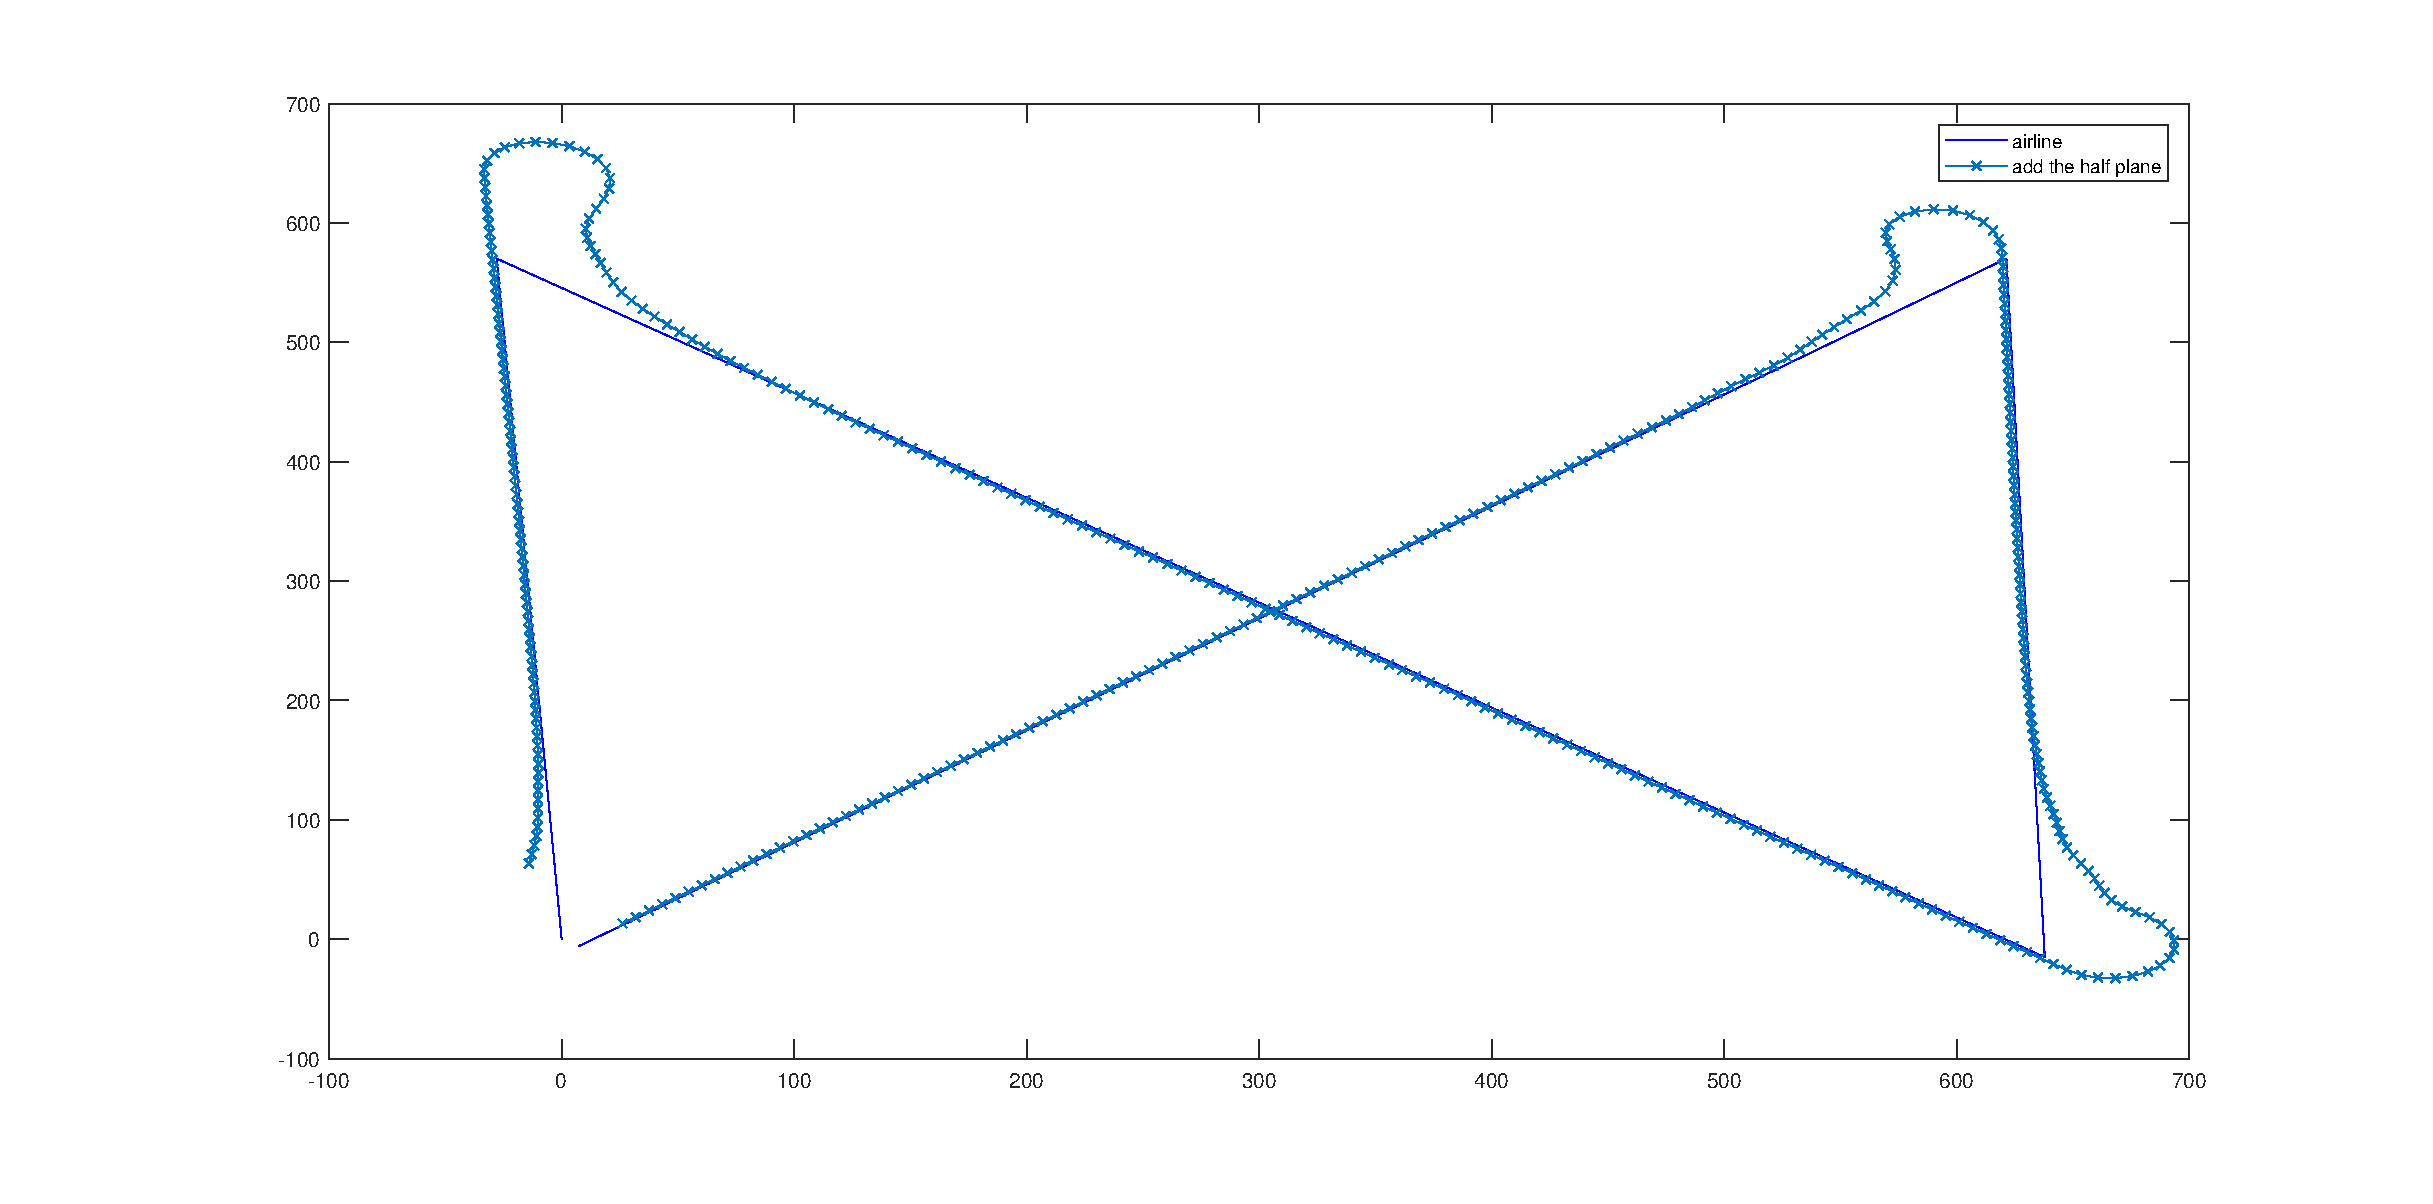
\includegraphics[width=\textwidth]{picture/eps/algorithm5.eps}
                \label{straight_}
            \end{minipage}
        }
        \caption{straight line}
    \end{figure}
    \begin{figure}[h]
        \centering
        \includegraphics[width=0.5\textwidth]{picture/algo6_2.png}
        \label{figure:alg6}
        \caption{插入fillet}
    \end{figure}
    \par 无人机从航点$w_{i-1}$到$w_{i}$的飞行过程中,若到达两条航线所生成的半平面,则认为到达了目标航点,航线进行切换。飞行控制逻辑包含直线飞行控制和盘旋飞行控制,在直线飞行的过程中,航点切换依附着算法\ref{algo5:ref}。
    
    第一次执行该算法时候,需要初始化i的值,让其等于2,见\ref{algo5:ref:init};UAV会执行航线$\overline{w_{i-1}w_{i}}$,在算法第4、5行分别定义针对当前执行航点的$r$和$q$,第6行定义了下一条航线的单位方向向量,第7行是航线 $\overline{w_{i-1}w_{i}}$ 和 $\overline{w_{i}w_{i+1}}$ 所生成半平面的法向量,8行到10行进行位置判定,若满足某个关系式,即若无人机穿过半平面,
    那么就要切换航点,执行下一条航线,直到最后一个航点序列号减一。
    \begin{algorithm}[h]
            \caption{Follow Waypoints:(r, q)=followWpp($\textit{W}$, p)}
            \label{algo5:ref}
            \begin{algorithmic}[1]
                \ENSURE Waypoints path $\textit{W}$ = $\left\{ w_{1}, \dots, w_{N} \right\}$, MAV position p=$(p_{n}, p_{e}, p_{d})^{T}$.
                \REQUIRE N $\geq$ 3
                \IF {New waypoints path $\textit{W}$ is received}
                    \STATE Initialize waypoint index: $i$ $\gets$ 2
                    \label{algo5:ref:init}
                \ENDIF
                \STATE $r$ $\gets$ $w_{i-1}$

                % \STATE $q_{i-1}$ $\gets$ $\frac{w_{i}-w_{i-1}}{\left \| w_{i}-w_{i-1} \right \|}$
                \STATE $q_{i-1}$ $\gets$ $\frac{w_{i}-w_{i-1}}{\lVert w_{i}-w_{i-1} \rVert}$
                \STATE $q_{i}$ $\gets$ $\frac{w_{i+1}-w_{i}}{\lVert w_{i+1}-w_{i} \rVert}$
                \STATE $n_{i}$ $\gets$ $\frac{q_{i-1}+q_{i}}{\lVert \| q_{i-1}+q_{i} \rVert}$
                \IF {$p$ $\in$ $\textit{H}(w_{i},n_{i})$}
                    \STATE Increment $i$ $\gets$ $\left(i+1\right)$ until $i$ = $N$ - 1
                \ENDIF
                \RETURN $r$, $q$=$q_{i-1}$ at each time step.  % this command shows "Output"
            \end{algorithmic}
        \end{algorithm}

        \par 算法\ref{algo5:ref}产生的飞行效果如图\ref{straight_}所示,
        很明显,但在直线飞行航点之间切换的时候,因忽略转弯时无人机初始动量的问题,造成了一段很长的转换缓冲距离,致使飞行效果很差,航线不平滑。
    \begin{figure}[h]
        \centering
        \includegraphics[width=0.6\textwidth]{picture/algo6_3.png}
        \label{algo6_1}
        \caption{将半平面和fillet进行结合}
    \end{figure}
    \par 一个较优的改进方法是为其增加一个圆角(fillet),如图5所示,在航点 $w_{i}$ 附近,生成一个盘旋中心,让其使得无人机在执行该航点的时候,以圆弧的方式进入到下一条航线,这么航线飞行出来的效果较好。定义航线$\overline{w_{i-1}w_{i}}$ 和$\overline{w_{i}w_{i+1}}$的角度为 $\varrho$:
    
    \begin{equation}
        \varrho \triangleq cos^{-1}(-q_{i-1}^{T}q_{i})
    \end{equation}
    
    \begin{algorithm}[h]
            \caption{Follow Waypoints with Fillet:(flag, r, q, c, $\rho$, $\lambda$)=followWppFillet($\textit{W}$, p, $R$)}
            \label{algo6:ref}
            \begin{algorithmic}[1]
                \ENSURE Waypoints path $\textit{W}$ = $\left\{ w_{1}, \dots, w_{N} \right\}$, MAV position p=$(p_{n}, p_{e}, p_{d})^{T}$, fillet radius $R$
                \REQUIRE N $\geq$ 3
                \IF {New waypoints path $\textit{W}$ is received}
                    \STATE Initialize waypoint index: $i$ $\gets$ 2, and state machine: state $\gets$ 1
                \ENDIF
                \STATE $q_{i-1}$ $\gets$ $\frac{w_{i}-w_{i-1}}{\lVert w_{i}-w_{i-1} \rVert}$
                \STATE $q_{i}$ $\gets$ $\frac{w_{i+1}-w_{i}}{\lVert w_{i+1}-w_{i} \rVert}$
                \STATE $\varrho$ $\gets$ $cos^{-1}(-q_{i-1}^{T}q_{i})$
                \IF {state = 1}
                    \STATE flag $\gets$ 1
                    \STATE $r$ $\gets$ $w_{i-1}$
                    \STATE $q$ $\gets$ $q_{i-1}$
                    \STATE $z$ $\gets$ $w_{i} - \frac{R}{tan(\frac{\varrho}{2})}q_{i-1}$

                    \IF {$p$ $\in$ $\textit{H}(z,q_{i-1})$}
                        \STATE state $\gets$ 2
                    \ENDIF
                \ELSIF{state = 2}
                    \STATE flag $\gets$ 2
                    \STATE $c$ $\gets$ $w_{i} - \frac{R}{sin(\frac{\varrho}{2})}\frac{q_{i-1}-q_{i}}{\lVert q_{i-1}-q_{i} \rVert}$
                    \STATE $\rho$ $\gets$ $R$
                    \STATE $\lambda$ $\gets$ $sign(q_{i-1,n}q_{i,e}-q_{i-1,e}q_{i,n})$
                    \STATE $z$ $\gets$ $w_{i} + \frac{R}{tan(\frac{\varrho}{2})}q_{i}$
                    \IF {$p$ $\in$ $\textit{H}(z,q_{i})$}
                        \STATE $i$ $\gets$ $\left(i+1\right)$ until $i$ = $N$ - 1
                        \STATE state $\gets$ 1
                    \ENDIF
                \ENDIF
                \RETURN flag, $r$, $q$, $c$, $\rho$,$\lambda$.  % this command shows "Output"
            \end{algorithmic}
        \end{algorithm}
在第\pageref{figure:alg6}页的图4中,假定fillet的半径为R,那么圆弧和两条航线的切点距航点$w_{i}$的距离为$\frac{R}{tan(\frac{\varrho}{2})}$
    且航点$w_{i}$和fillet的中心的距离是$\frac{R}{sin(\frac{\varrho}{2})}$,所以航点$w_{i}$距圆角fillet的最短距离为$\frac{R}{sin(\frac{\varrho}{2})}$ - $R$.
    为了让其直线控制逻辑和圆弧控制逻辑\upcite{8}更好的结合,对此也引进来了"半平面"。
    在第\pageref{algo6_1}页的图5中,
    定义了两个半平面 \textit{$H_{1}$} 和 \textit{$H_{2}$}。飞机在未进入半平面 \textit{$H_{1}$}
    的时候,执行直线控制逻辑;当进入到 \textit{$H_{1}$} 的时候,执行圆弧控制逻辑,此时,圆弧的中心是 $c$,半径是 $\rho$;直到无人机进入 \textit{$H_{2}$} ,切换到直线控制逻辑。
    在算法\ref{algo6:ref}中,给出了详细的逻辑梳理。
    圆角的中心 $c$, 第一个半平面、第二半平面与圆角相交的点 $r_{1}$ 和 $r_{2}$ 定义如下:
        \begin{align}
            &c = w_{i} - \frac{R}{sin(\frac{\varrho}{2})} \frac{q_{i-1}-q_{i}}{\lVert q_{i-1}-q_{i} \rVert} \\
            &r_{1} = w_{i} - \left( \frac{R}{tan(\frac{\varrho}{2})} \right)q_{i-1} \\
            &r_{2} = w_{i} + \left( \frac{R}{tan(\frac{\varrho}{2})} \right)q_{i}
        \end{align}
    \par其中的向量 $q_{i-1}$ 和 $q_{i}$ 分别为两条航线的单位方向向量。算法\ref{algo6:ref}中,若一条新的航线被接收,那么航点序列号和state的值也会在第2行进行更新,向量$q_{i-1}$ 和 $q_{i}$,以及$\varrho$在4到6行计算;
    当state = 1的时候,调用直线控制逻辑,执行航线 $\overline{w_{i-1}w_{i}}$,同时计算相对应的 $r$ 和 $q$,在第11到14行判断是否到达第一个半平面;若无人机穿过第一个半平面,朝着第二个半平面飞去的时候,state = 2,执行曲线控制逻辑,对应的圆心为$c$,半径为$\rho$,飞行的方向(逆时针,或顺时针)为$\lambda$;若无人机穿过第二个半平面,则state赋值为1,执行直线控制逻辑。

    
    \section{算法优化} 
    算法\ref{algo5:ref}和算法\ref{algo6:ref}执行效果对比如图\ref{algo5_com_6}所示, 图\ref{5_6_bigger}是将右下角转弯轨迹放大之后得到的. 很显然, 从总体路径长度最优的角度来看, 后者的总体路径长度要明显比前者总体路径长度短很多, 执行效率也会优于前者.
    \begin{figure}[h]
        \centering
        \subfigure[]{
            \begin{minipage}[t]{0.48\linewidth}
                \centering
                    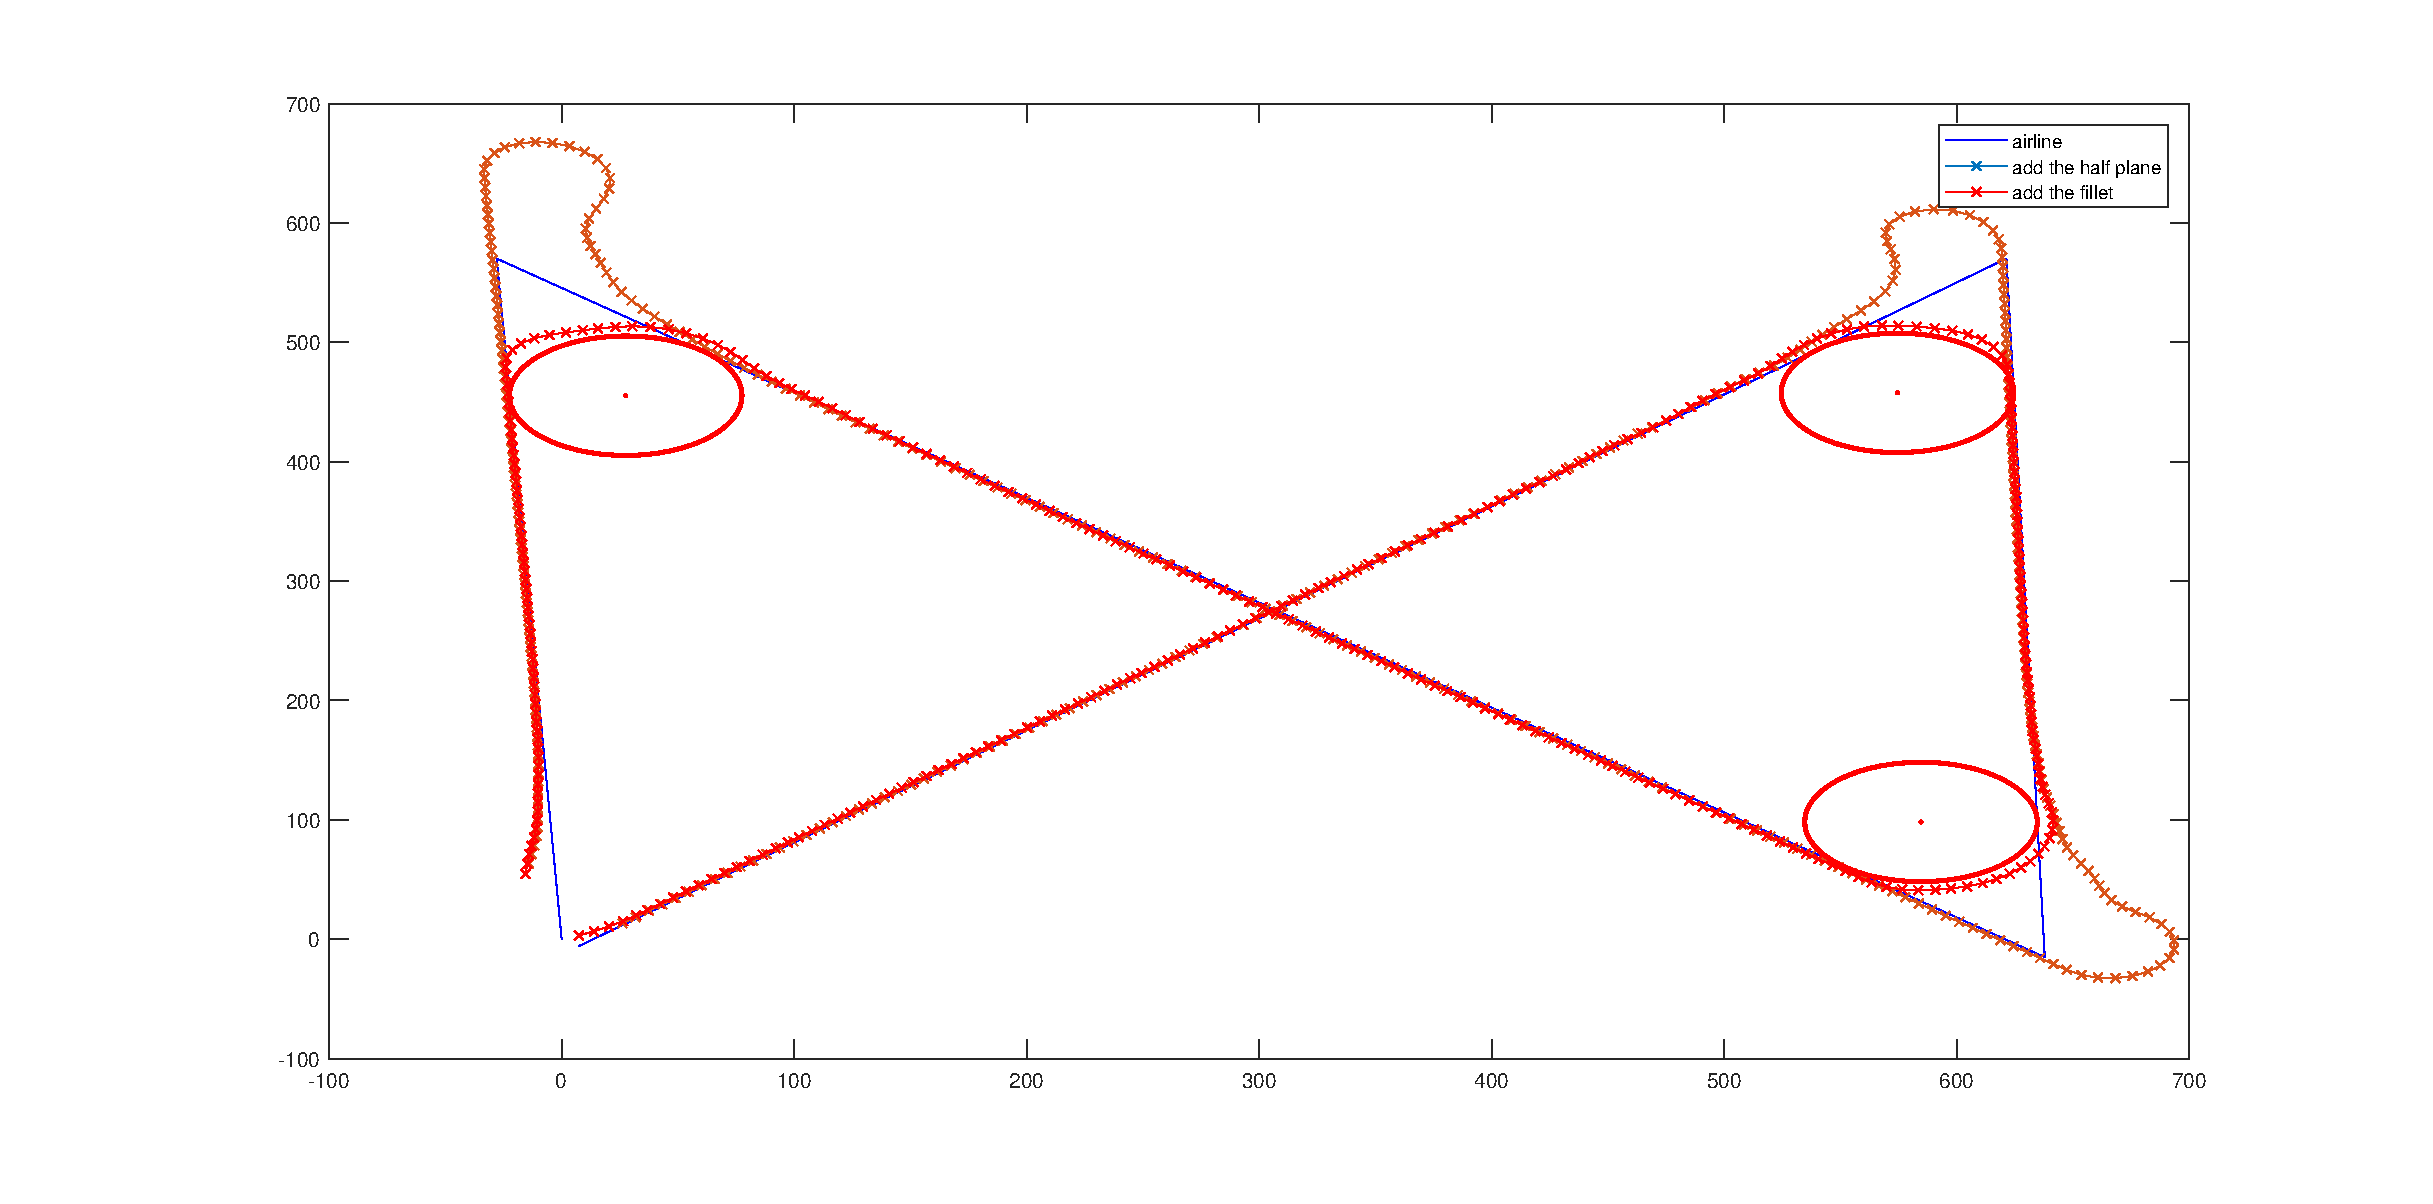
\includegraphics[width=\textwidth]{picture/eps/algorithm5_6.eps}
                \label{algo5_com_6}
            \end{minipage}
        }
        \subfigure[]{
            \begin{minipage}[t]{0.48\linewidth}
                \centering
                    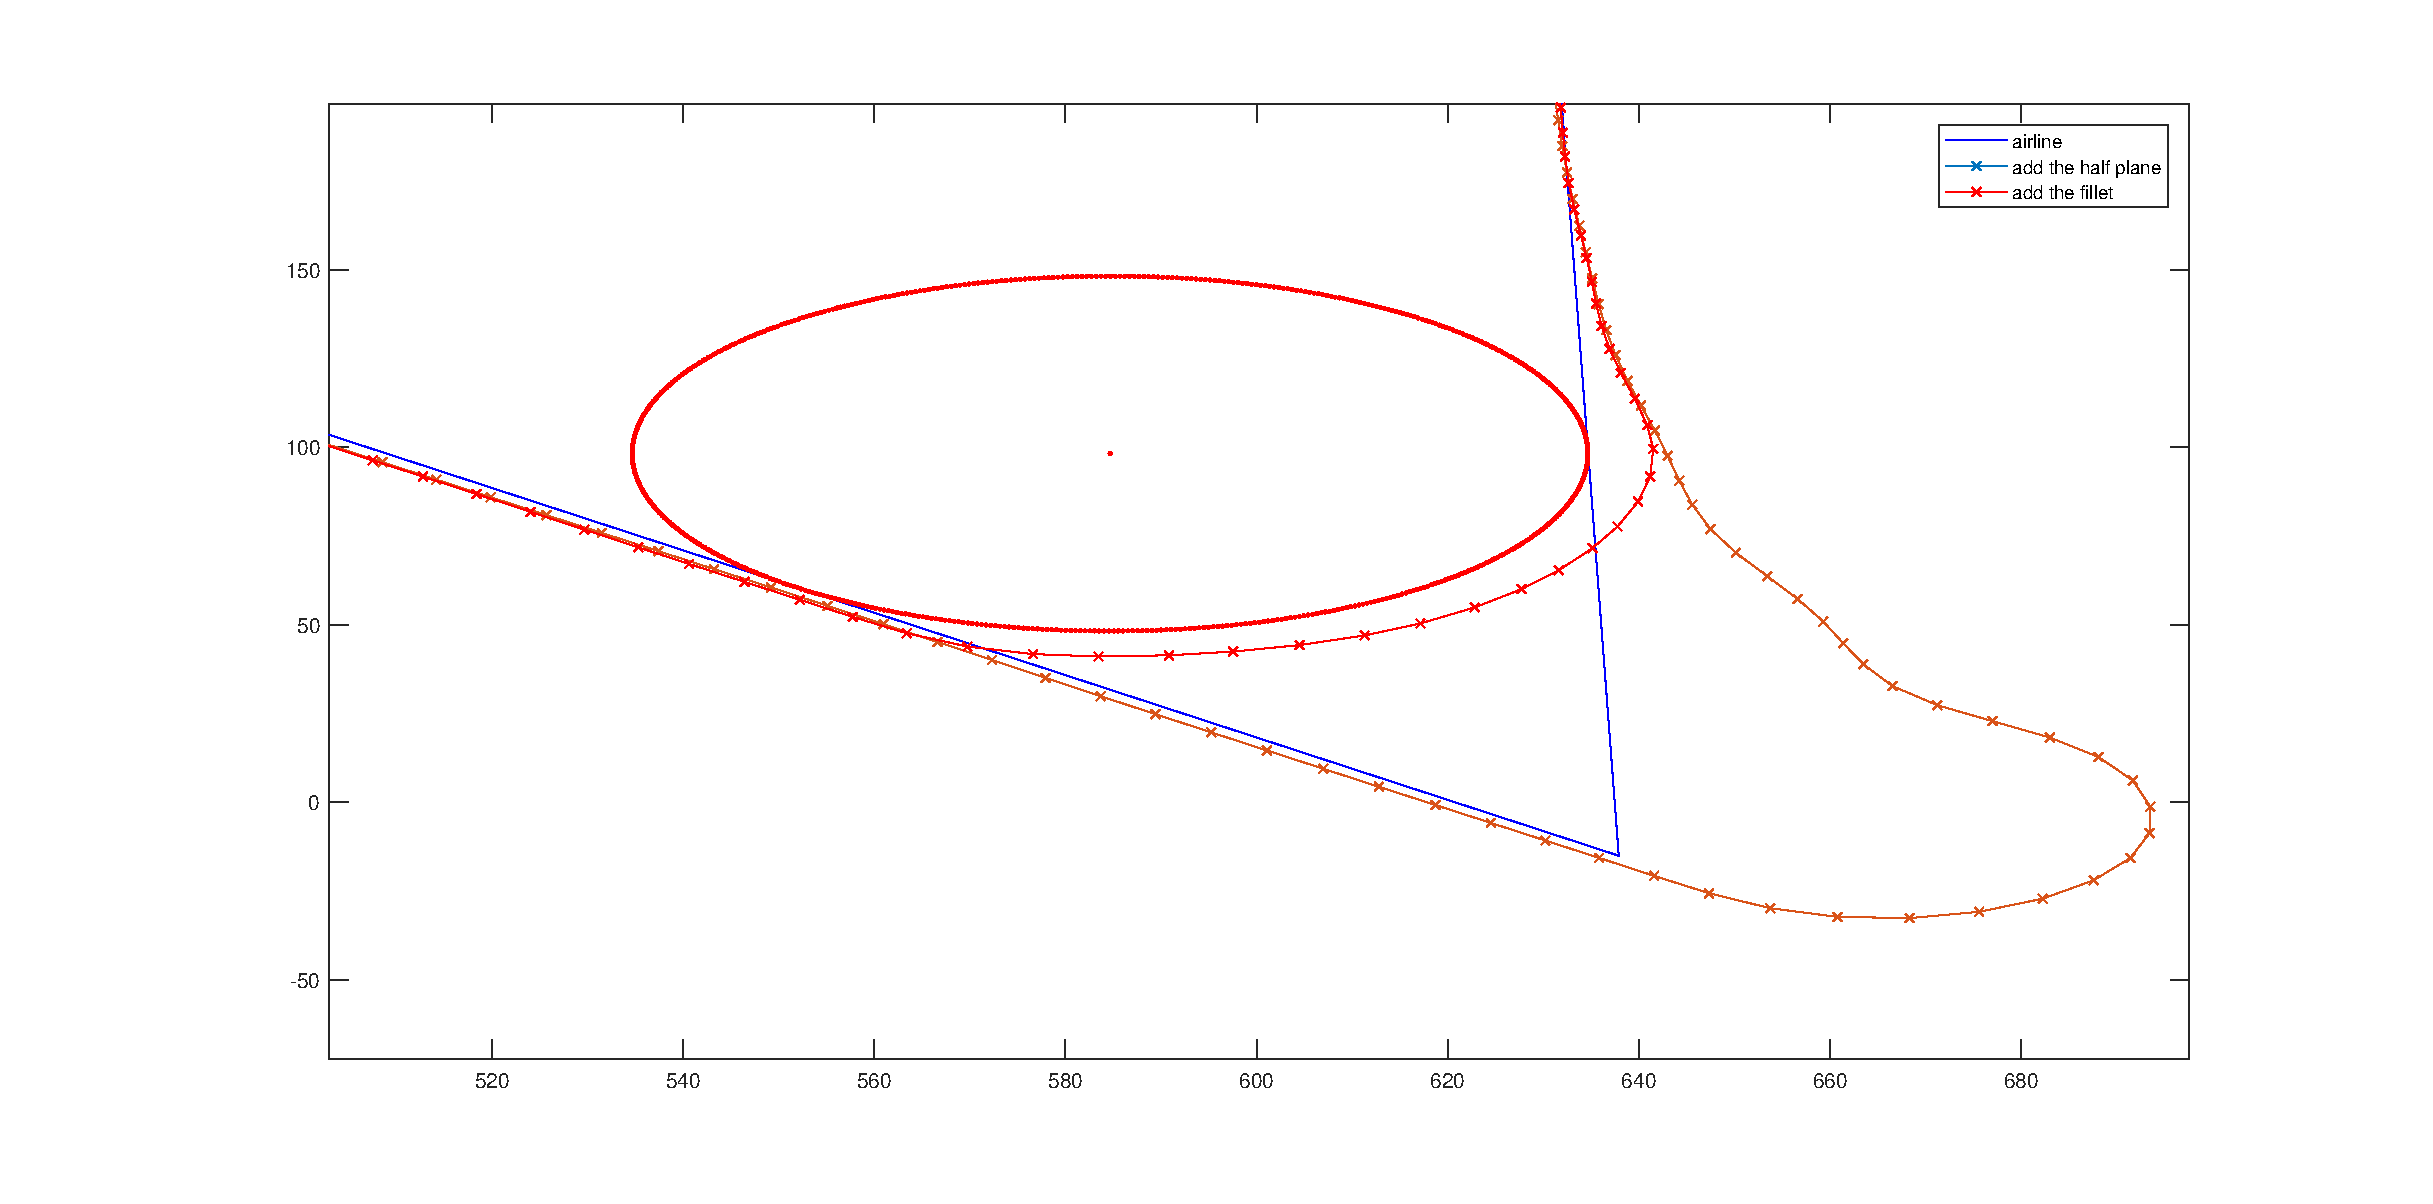
\includegraphics[width=\textwidth]{picture/eps/algorithm5_6_1.eps}
                \label{5_6_bigger}
            \end{minipage}
        }
        \caption{comparing}
    \end{figure}
    尽管如此, 算法\ref{algo6:ref}在转弯的时候, 对初试惯性动量考虑的不太周到, 存在一些瑕疵, 如图\ref{fig:algo6}所示.
    虽然在算法\ref{algo6:ref}中, 模型建立是以fillet和航线相切的情况来考虑的, 但在仿真平台中, 无人机的并不是以期望空速来飞行, 而是以期望空速(airspeed)和风速(wind speed)叠加之后形成的地速(ground speed)来飞行. 由于风速大小的不确定性, 造成了飞行效果差强人意.
    \begin{figure}[htbp]
        \centering
        \subfigure[]{
            \begin{minipage}[t]{0.48\linewidth}
                \centering
                    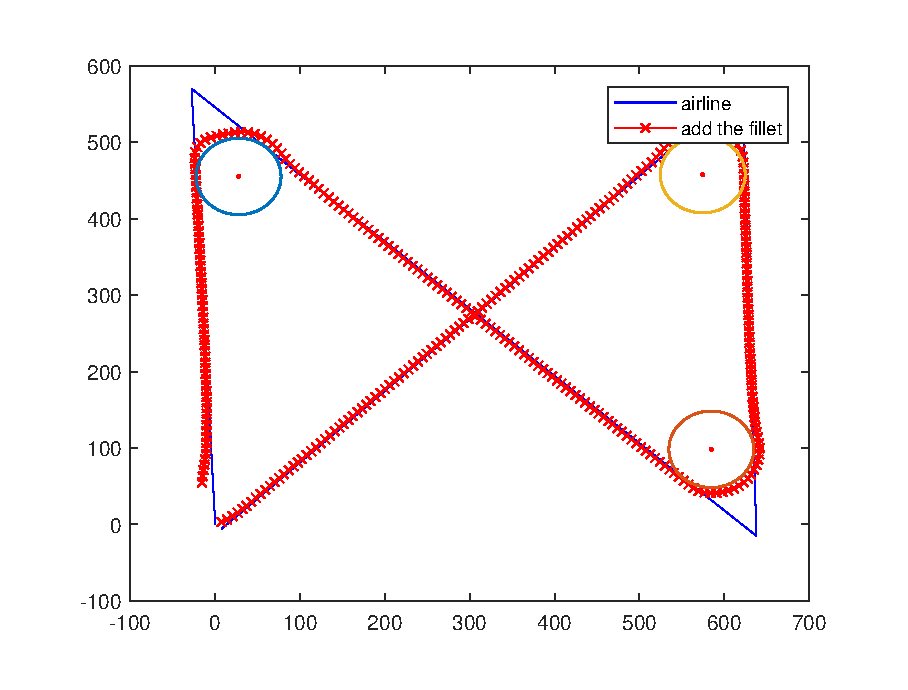
\includegraphics[width=0.8\textwidth]{picture/eps/algorithm6.eps}
                \label{fig:algo6}
            \end{minipage}
        }
        \subfigure[]{
            \begin{minipage}[t]{0.48\linewidth}
                \centering
                    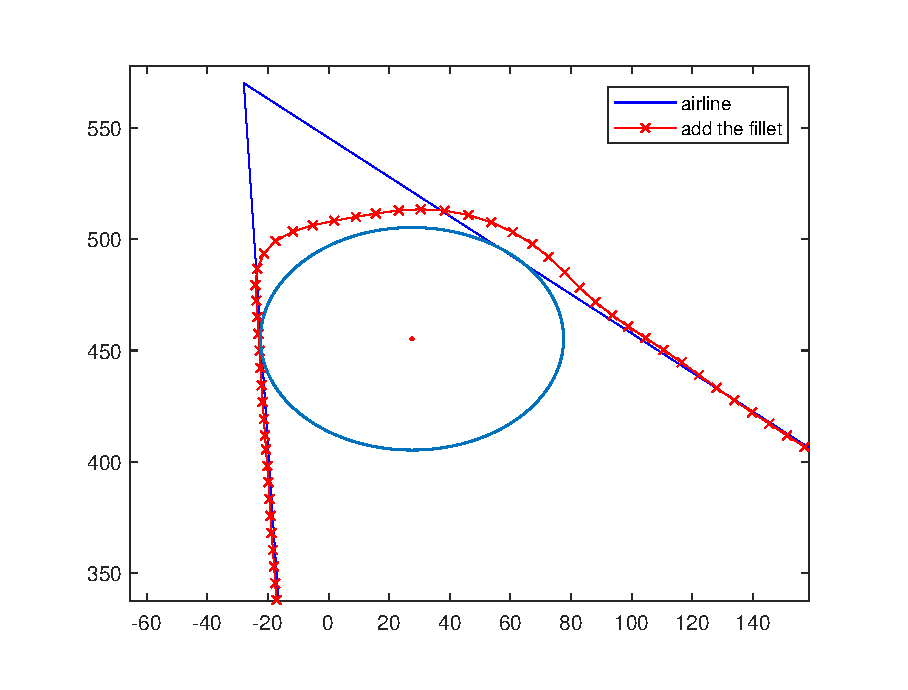
\includegraphics[width=0.8\textwidth]{picture/eps/algorithm6_1.eps}
                \label{fig:algo6_1}
            \end{minipage}
        }
        \\
        \subfigure[]{
            \begin{minipage}[t]{0.48\linewidth}
                \centering
                    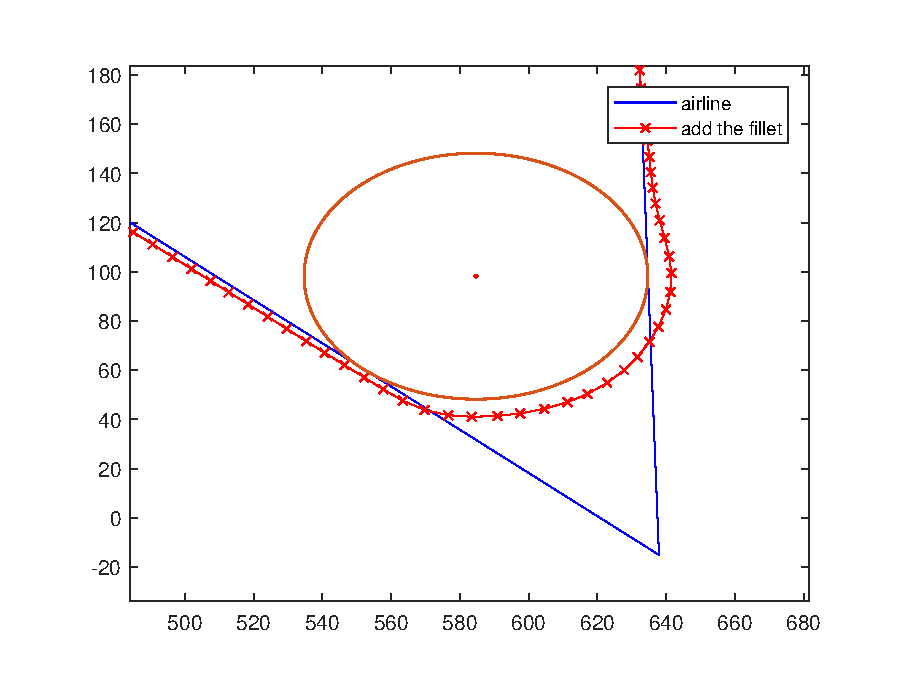
\includegraphics[width=0.8\textwidth]{picture/eps/algorithm6_2.eps}
                \label{fig:algo6_2}
            \end{minipage}
        }
        \subfigure[]{
            \begin{minipage}[t]{0.48\linewidth}
                \centering
                    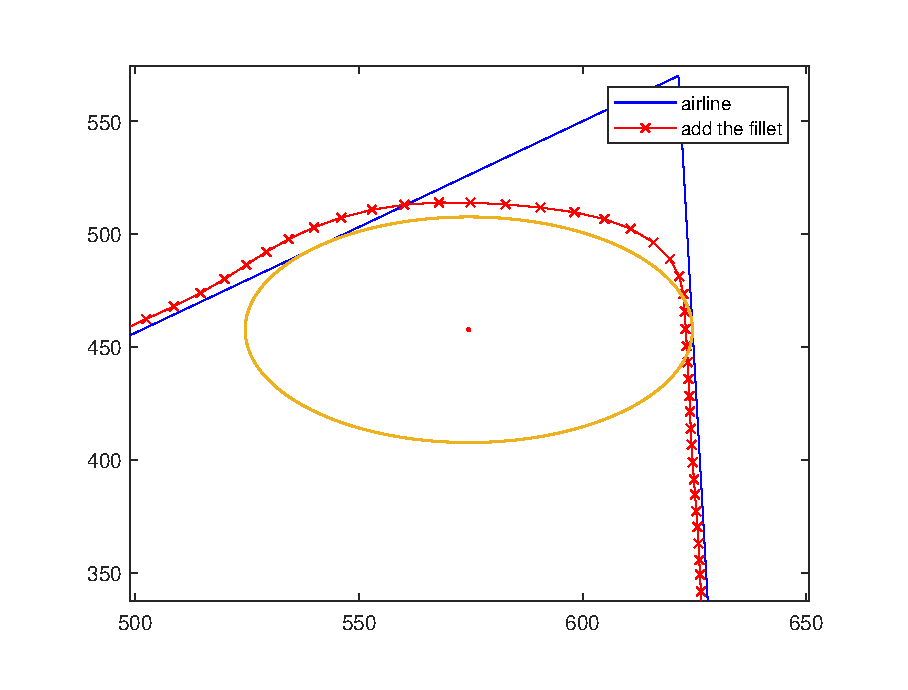
\includegraphics[width=0.8\textwidth]{picture/eps/algorithm6_3.eps}
                \label{fig:algo6_3}
            \end{minipage}
        }
        \caption{algorithm6}
    \end{figure}
 
    对此提出了一个算法的改进. 根据图\ref{fig:algo6_1}, \ref{fig:algo6_2}, \ref{fig:algo6_3}显示, 超出航线的那一小部分还是由于惯性动量导致的, 所以在这里我们需要提前来进行航先切换, 从而留出一部分来减弱惯性动量, 让转弯轨迹更加的圆滑, 航线执行总的距离更小. 故对算法\ref{algo6:ref}进行了改进, 从而得到了算法\ref{algo6_opti:ref}.   
    \begin{figure}[htbp]
        \centering
        \subfigure[]{
            \begin{minipage}[t]{0.48\linewidth}
                \centering
                    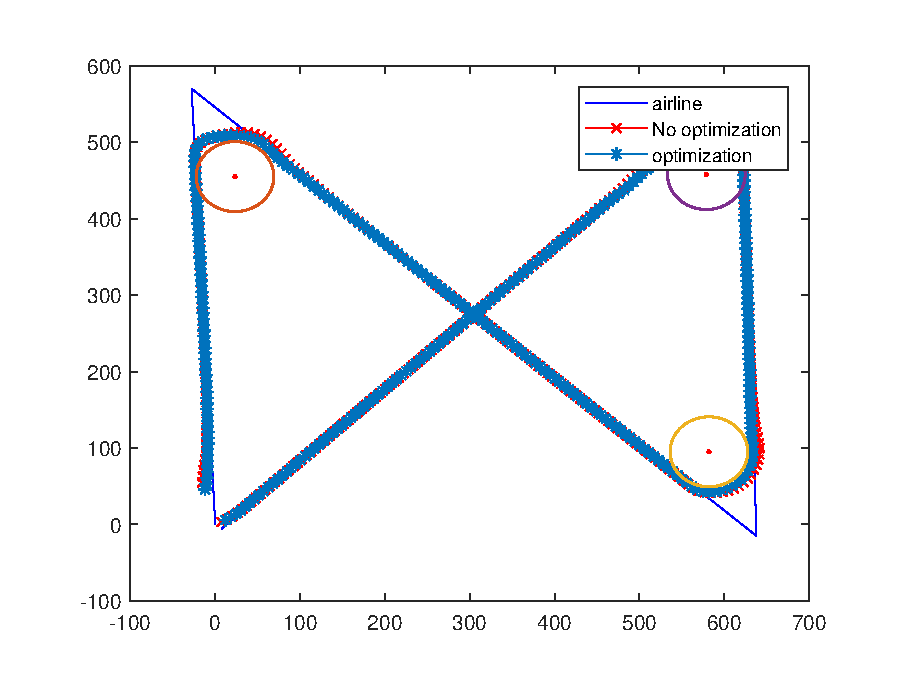
\includegraphics[width=0.7\textwidth]{picture/eps/algorithm7.eps}
                \label{fig:algo7}
            \end{minipage}
        }
        \subfigure[]{
            \begin{minipage}[t]{0.48\linewidth}
                \centering
                    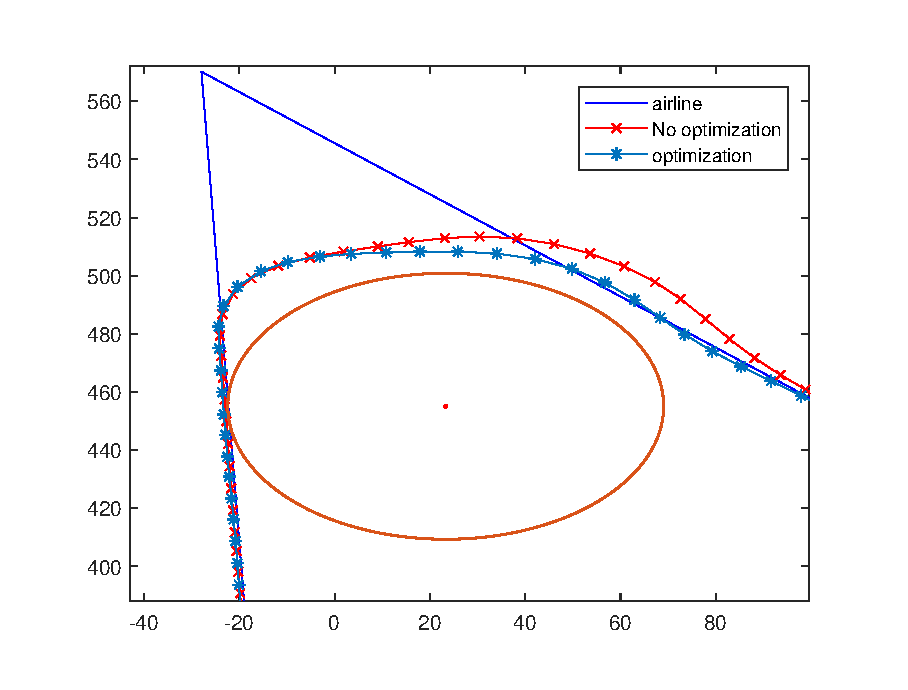
\includegraphics[width=0.7\textwidth]{picture/eps/algorithm7_1.eps}
                \label{fig:algo7_1}
            \end{minipage}
        }
        \\
        \subfigure[]{
            \begin{minipage}[t]{0.48\linewidth}
                \centering
                    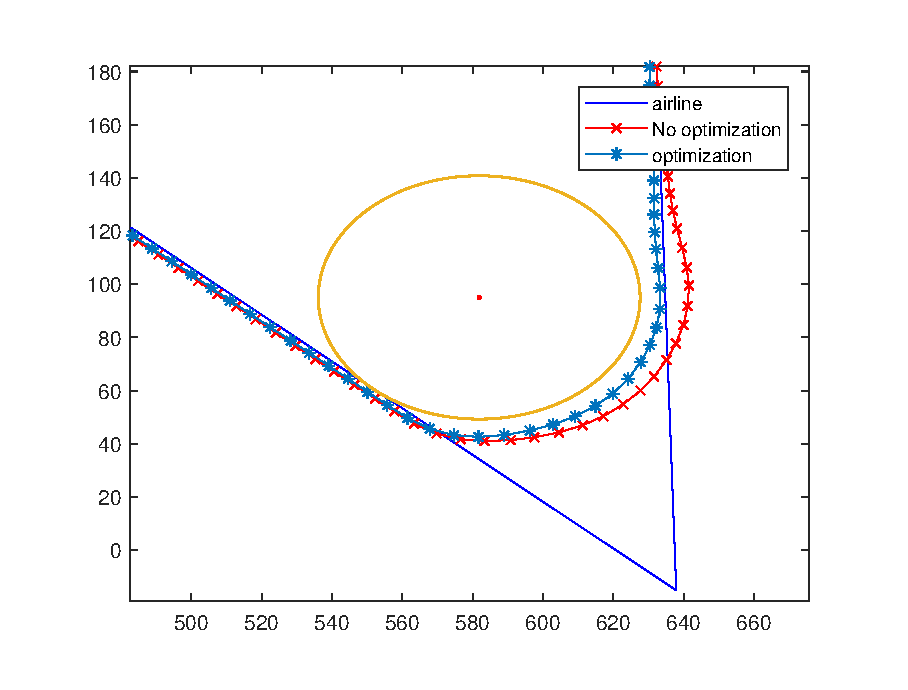
\includegraphics[width=0.7\textwidth]{picture/eps/algorithm7_2.eps}
                \label{fig:algo7_2}
            \end{minipage}
        }
        \subfigure[]{
            \begin{minipage}[t]{0.48\linewidth}
                \centering
                    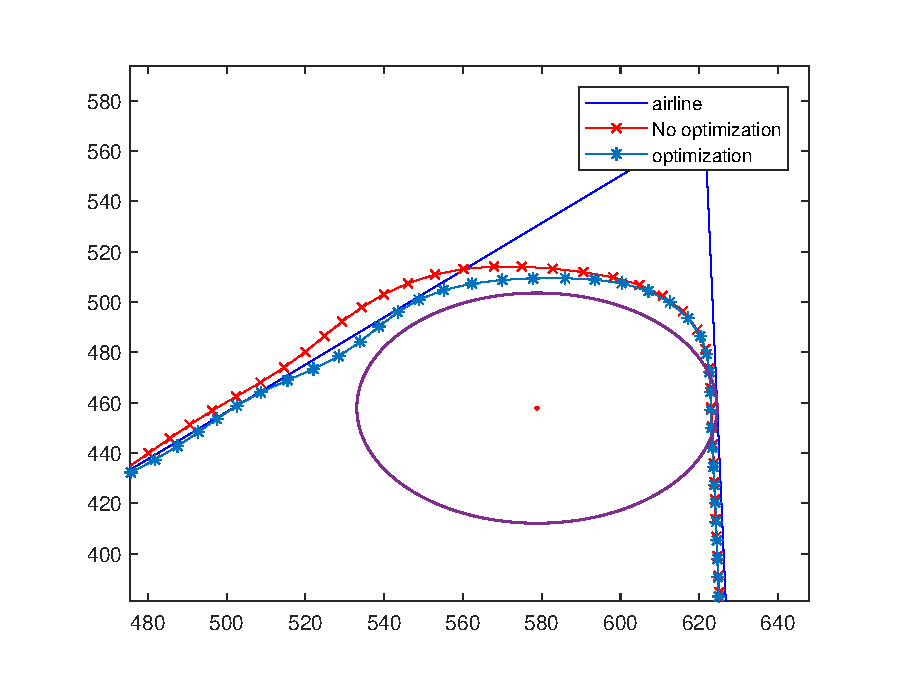
\includegraphics[width=0.7\textwidth]{picture/eps/algorithm7_3.eps}
                \label{fig:algo7_3}
            \end{minipage}
        }
        \caption{algorithm6 comparing 1}
    \end{figure}
    
    \par 算法中, 在\ref{algo7_z1}行, 保存第一个半平面与航线$\overline{w_{i-1}w_{i}}$的交点$z$为$z_{1}$, 
    当进入第一个半平面的时候,state = 2,执行曲线控制逻辑,对应的圆心为第\ref{new_center}行所示的$c$, 其中半径进行了一定比例的缩放,已到达保留一定的距离来消耗无人机初始惯性动量的目的。第20行和22行,对应的R都进行了比例缩放,其中第20行是为fillet center设置半径,第22行是计算新的第二个半平面和下一条航线的新交点;第23行判断是否到达第二个半平面,若到达则切换航线,state重新设置为1,执行直线控制逻辑;反之继续执行当前航线。
    前后算法比对的效果图如图\ref{fig:algo7}所示。
    \begin{algorithm}[t] % 算法6 的优化
        \caption{Follow Waypoints with Fillet:(flag, r, q, c, $\rho$, $\lambda$)=followWppFillet($\textit{W}$, p, $R$)}
        \label{algo6_opti:ref}
        \begin{algorithmic}[1]
            \ENSURE Waypoints path $\textit{W}$ = $\left\{ w_{1}, \dots, w_{N} \right\}$, MAV position p=$(p_{n}, p_{e}, p_{d})^{T}$, fillet radius $R$
            \REQUIRE N $\geq$ 3
            \IF {New waypoints path $\textit{W}$ is received}
                \STATE Initialize waypoint index: $i$ $\gets$ 2, and state machine: state $\gets$ 1
            \ENDIF
            \STATE $q_{i-1}$ $\gets$ $\frac{w_{i}-w_{i-1}}{\lVert w_{i}-w_{i-1} \rVert}$
            \STATE $q_{i}$ $\gets$ $\frac{w_{i+1}-w_{i}}{\lVert w_{i+1}-w_{i} \rVert}$
            \STATE $\varrho$ $\gets$ $cos^{-1}(-q_{i-1}^{T}q_{i})$
            \IF {state = 1}
                \STATE flag $\gets$ 1
                \STATE $r$ $\gets$ $w_{i-1}$
                \STATE $q$ $\gets$ $q_{i-1}$
                \STATE $z$ $\gets$ $w_{i} - \frac{R}{tan(\frac{\varrho}{2})}q_{i-1}$
                \STATE $z_{1}$ $\gets$ $z$     \label{algo7_z1}   
                \IF {$p$ $\in$ $\textit{H}(z,q_{i-1})$}
                    \STATE state $\gets$ 2
                \ENDIF
            \ELSIF{state = 2}
                \STATE flag $\gets$ 2
                
                % 计算新的 center >>>>>>>>>>>>>>>>> 
                \STATE $c$ $\gets$ $w_{i} - \frac{R}{sin(\frac{\varrho}{2})}\frac{q_{i-1}-q_{i}}{\lVert q_{i-1}-q_{i} \rVert}$
                \STATE $c$ $\gets$ $z_{1} + \frac{c-z_{1}}{\lVert c-z_{1}\rVert}*0.915R$ %  \frac{R}{sin(\frac{\varrho}{2})}\frac{q_{i-1}-q_{i}}{\lVert \| q_{i-1}-q_{i} \rVert}$
                \label{new_center}
                \STATE $\rho$ $\gets$ $0.915R$
                % <<<<<<<<<<<<<<<<< 计算新的 center

                \STATE $\lambda$ $\gets$ $sign(q_{i-1,n}q_{i,e}-q_{i-1,e}q_{i,n})$
                \STATE $z_{2}$ $\gets$ $w_{i} + \frac{1}{tan(\frac{\varrho}{2})}*0.915R*q_{i}$
                \IF {$p$ $\in$ $\textit{H}(z,q_{i})$}
                    \STATE $i$ $\gets$ $\left(i+1\right)$ until $i$ = $N$ - 1
                    \STATE state $\gets$ 1
                \ENDIF
            \ENDIF
            \RETURN flag, $r$, $q$, $c$, $\rho$,$\lambda$.  % this command shows "Output"
        \end{algorithmic}
    \end{algorithm}
    \subsection{误差分析}
    \begin{center} 
        \begin{table}[H]
            \caption{误差分析表}
            \label{tab1}
            \begin{tabular}{c|c|c|c|c}
                \hline
                & 第一段(*150)& 第二段((*130))& 第三段(*120) &总和 \\
                \hline
                优化之前 &9.506485437269829& 13.459338133308067& 12.517388189403794 & 11.694433389122446 \\
                \hline
                优化之后 &9.307437579575690& 2.896129449605189& 7.097844734906930 & 6.560884583934650 \\
                \hline
                % \caption{误差分析表}
            \end{tabular} 
        \end{table}   
    \end{center}
    
    通过计算超出航线部分的点到航线的垂直距离,即偏离航线的误差,来判定算法是否优化。算法优化之前和优化之后误差分析如\ref{tab1}所示。
    最终计算得到的总的偏差由11.7减少到6.6,效果优化了78\%,足以可见算法\ref{algo6_opti:ref}较之前算法具有很好的效用性。
    \clearpage

    \section{结 论}
    针对无人机飞行控制逻辑有两种:直线控制逻辑和曲线控制逻辑。无论哪种控制逻辑,都会涉及到航点航线之间的切换时刻。
    直线控制中,可以设定当无人机和航线满足一定要求的时候,进行航点切换,比如:当无人机的当前位置在当前航线上的映射比例大于设定值时,进行切换航点;当无人机穿过提前设定好的转弯平面时,进行航线切换等。
    本文主要是在后者的逻辑上,要解决特定算法在转弯的时候,航线轨迹太长的问题。方法是通过为其留出一定的距离来消耗转弯的初始惯性动量,来减少惯性,从而达到减小航线总长度的目标,使得无人机执行任务更加高效,能源消耗的更慢。
    实验结果表明:算法改进之后具有很好的高效性,能很大程度的减小偏差。    
    \clearpage % 分页
%     \bibliographystyle{unsrt}   % unsrt 为文献的格式类型
% \bibliography{mysef} % mysef 为我们的.bib文件名


\addcontentsline{toc}{section}{参考文献}
\renewcommand{\refname}{参考文献}
\begin{thebibliography}{99}
\addtolength{\itemsep}{-2ex} % 用于更改行距
\bibitem{1}杨玉,金敏,鲁华祥.融合简化稀疏A*算法与模拟退火算法的无人机航迹规划[J].计算机系统应用,2019,28(4):25-31. DOI:10.15888/j.cnki.csa.006864.
\bibitem{2}张岳平,朱力超,孙涛.用Hopfield神经网络与模拟退火算法求解UAV航路规划问题[J].海军航空工程学院学报,2007,22(4):451-453,466. DOI:10.3969/j.issn.1673-1522.2007.04.012.
\bibitem{3}赵梵喆,林跃,杨永琪.基于多目标规划的无人机路径规划[J].价值工程,2020,39(9):208-210.
\bibitem{4}谭若晨.基于Multi-Agent系统的多UAV实时路径规划研究与实现[D].四川:电子科技大学,2013. DOI:10.7666/d.D772105.
\bibitem{5}耿兴元.基于GPS与GIS的导航系统研究与开发[D].浙江:浙江大学,2004.
\bibitem{6}张帅, 李学仁, 张鹏, 等.基于改进 A* 算法的无人机航迹规划[J] .飞行力学, 2016, 34( 3) : 39-43.
\bibitem{7}Liu LF, Shi RX, Li SD, et al. Path planning for UAVS based
on  improved  artificial  potential  field  method  through
changing  the  repulsive  potential  function.  Proceedings  of
2016  IEEE  Chinese  Guidance,  Navigation  and  Control
Conference  (CGNCC).  Nanjing,  China.  2016.  2011–2015.
\bibitem{8}D. R. Nelson, D. B. Barber, T. W. McLain and R. W. Beard, "Vector field path following for small unmanned air vehicles," 2006 American Control Conference, Minneapolis, MN, 2006, pp. 7 pp.-, doi: 10.1109/ACC.2006.1657648.
\bibitem{9}Randal W. Beard and Timothy W. McLain, "Small Unmanned Aircraft: Theory and Practice", 2012, Princeton University Press
\bibitem{10}R. W. {Beard} and T. W. {McLain} and D. B. {Nelson} and D. {Kingston} and D. {Johanson}, "Decentralized Cooperative Aerial Surveillance Using Fixed-Wing Miniature {UAVs}", 2006, Proceedings of the IEEE, 94, 7, 1306-1324
\bibitem{11}R. W. {Beard} and J. {Ferrin} and J. {Humpherys}, "Fixed Wing {UAV} Path Following in Wind With Input Constraints", 2014, IEEE Transactions on Control Systems Technology, 2014, 22, 6, 2103-2117
\bibitem{12}S. {Fari} and X. {Wang} and S. {Roy} and S. {Baldi}, "Addressing Unmodelled Path-Following Dynamics via Adaptive Vector Field: a {UAV} Test Case", 2019, IEEE Transactions on Aerospace and Electronic Systems, 10.1109/TAES.2019.2925487
\end{thebibliography}  
\clearpage
\end{document}
